\documentclass[a0,landscape]{a0poster}
% pdfLaTeX template
% For use with  CECS A0 poster presentations
% By James Ashton 2010-04-06
\usepackage{CECSposter}                % Define Title and section header appearance
\usepackage{graphicx}                  % Allow the inclusion of graphics
\usepackage{flowfram}                  % Flow frame package
\usepackage{url}
\usepackage{wrapfig}
\usepackage{subfigure}
\usepackage{cite}
%\usepackage{aaai}
%
\usepackage{winfonts}                  % Facilitate the use of fonts from Microsoft Windows
\pdfmapfile{+winfonts.map}             % tell pdftex where to find the fonts
\usepackage[T1]{fontenc}               % we need T1 encoding for this to work
\renewcommand{\familydefault}{tahoma}  % ANU says to use Tahoma when we don't have Rotis
%
\addtolength{\oddsidemargin}{20bp}     % Increase the margins on
\addtolength{\textwidth}{-70bp}        % all four sides to allow
\addtolength{\textheight}{-240bp}      % for the space taken up
\addtolength{\topmargin}{-30bp}        % by the red CECS frame.
\makebackgroundframe                   % Background static frame used by the red CECS frame
%
% The following code can (and probably should) be changed to suit each individual
% poster.  This is just an example of what can be done with flowfram.  There's
% a title frame at the top with four, equal-width column frames below.  We need to
% shorten the leftmost column to allow for the way the ANU logo protrudes in from
% the CECS frame.  Also, we have a double width figure frame below the middle two
% columns.
%
\setlength{\vcolumnsep}{30bp}          % 30 big points between columns vertically
\setlength{\columnsep}{60bp}           % 60 big points between columns horizontally
\Ncolumntop{static}{3}{150bp}          % Make 1 static and 4 flow frames
\setstaticframe{1}{label={title}}      % Call the static frame `title'
\newlength\wideheight
\setlength{\wideheight}{15in}          % How high will our double width frame be?
\newlength\offset                      % The offset up to the bottom of the middle columns
\setlength{\offset}{\wideheight}       % is the height of the wide frame
\addtolength{\offset}{\vcolumnsep}     % plus the vertical column separation
\computeflowframearea{1,2}
\newlength\leftheight
\setlength{\leftheight}{\ffareaheight}
\addtolength{\ffareaheight}{-\offset}  % reduce the middle column heights by the offset
\newlength\logooffset
\setlength{\logooffset}{0mm}           % Height of ANU logo above the rest of the border
\setflowframe{1}{width=12in}
\setflowframe{2}{x=13in, width=18in}
\setflowframe{3}{x=35in, width=12in}
\addtolength{\leftheight}{-\logooffset} % leave space for ANU logo
\setflowframe{1}{y=1in,height=23in}
\setflowframe{2}{y=1in, height=23in}
\setflowframe{3}{y=1in,height=23in}

%\newstaticframe{\ffareawidth}{\wideheight}{11.25in}{13.5in}[figure]
%\newstaticframe{\ffareawidth}{6.5in}{11in}{0in}[results]
\newstaticframe{\ffareawidth}{2in}{27.2in}{25.5in}[nicta]
%\setstaticframe{2}{clear}
\setallflowframes{border=none}
\setallstaticframes{border=none}
\title{Fast and Optimal Pathfinding on Grid Maps}
\date{}% Don't show the date
\author{Daniel Harabor \and Adi Botea}
\begin{document}
\begin{staticcontents*}{title}
\maketitle
\end{staticcontents*}
\thispagestyle{empty} 


% this just fills the empty columns
%\framebreak\mbox{}%\framebreak\mbox{}
\setstaticcontents{1}{
\includegraphics{CECSframe}}
%\begin{staticcontents*}{figure}
%\begin{staticfigure}
%\label{fig:splash}
%\begin{center}
%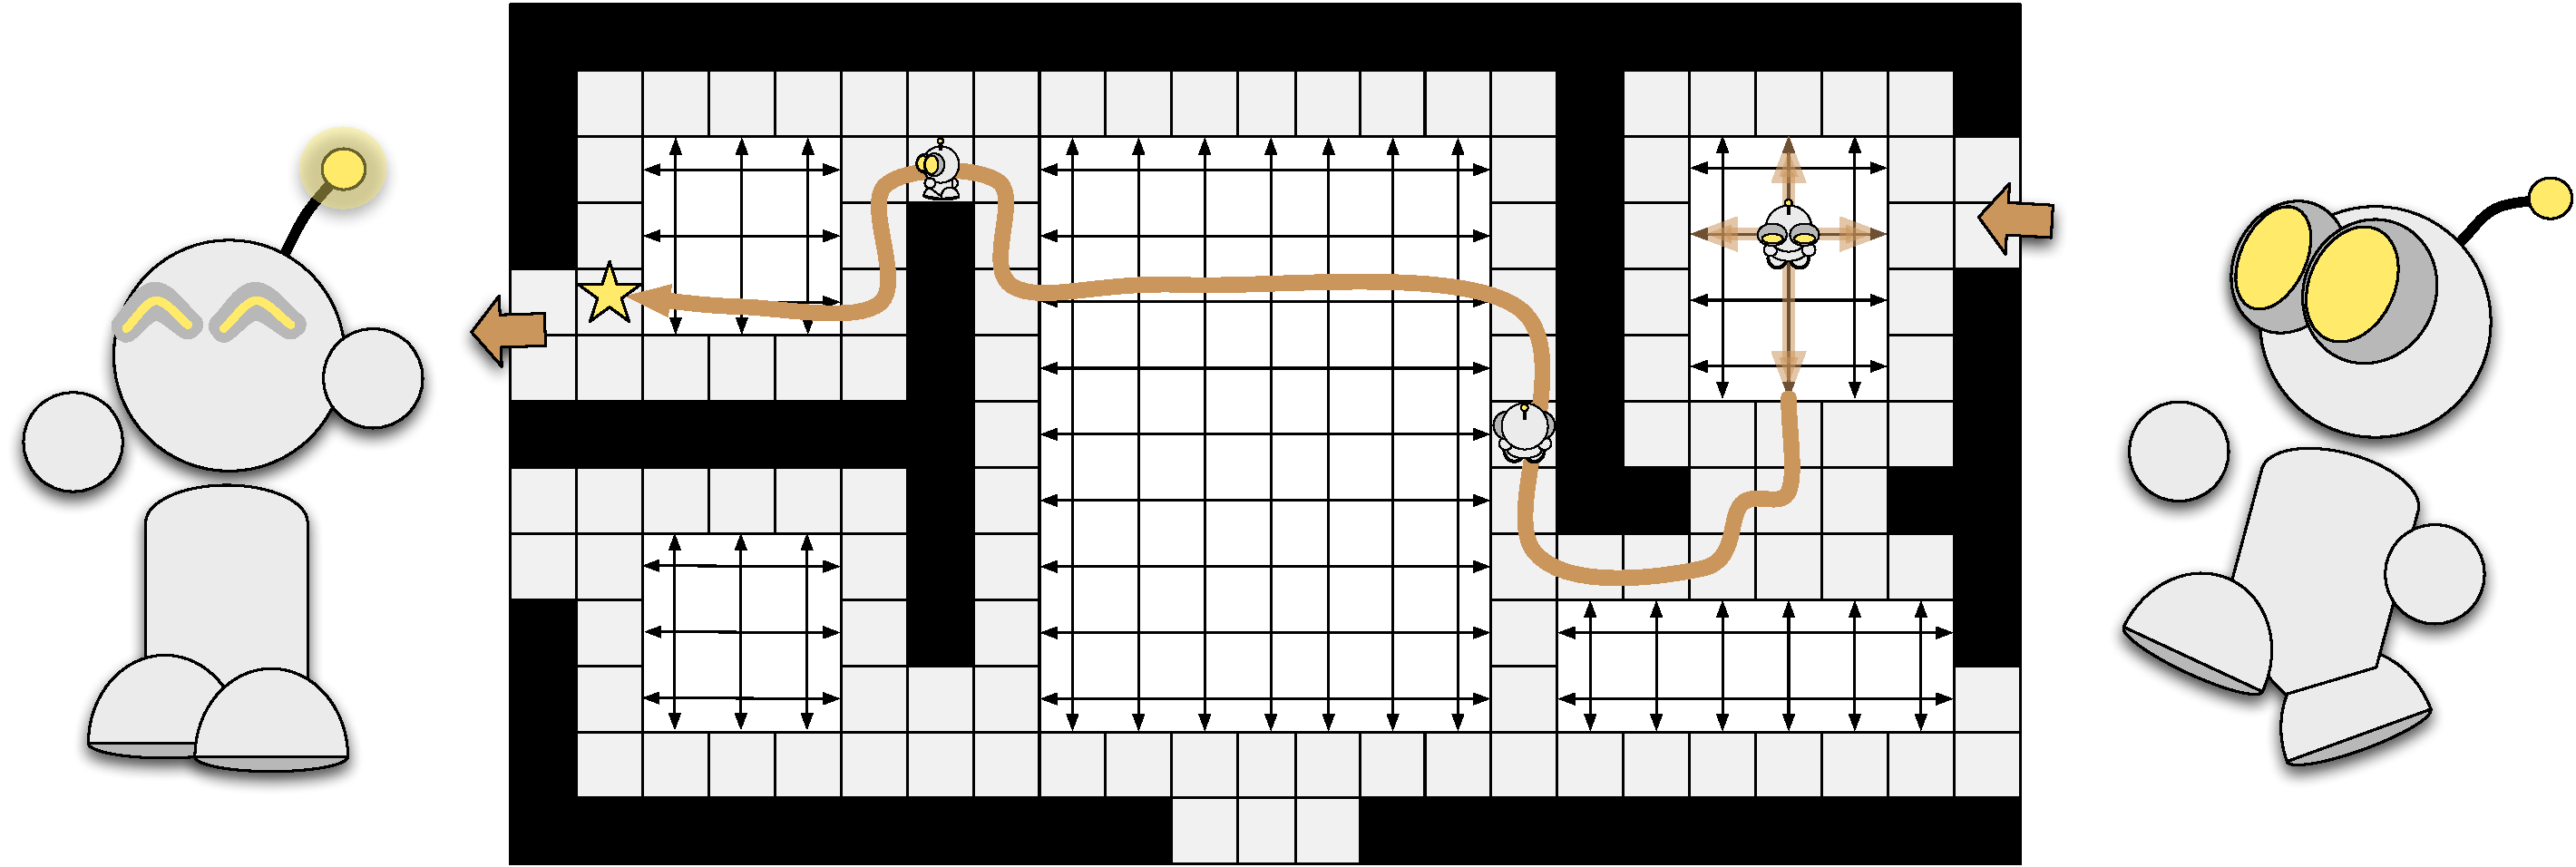
\includegraphics[width=\textwidth]{diagrams/robot_splash2}
%\caption{We speed up search by decomposing a 4-connected map into rectangular
%rooms which can be traversed without visiting any tiles from their interior.} 
%\end{center}
%\end{staticfigure}
%\end{staticcontents*}
%
%\begin{staticcontents*}{results}
%\begin{staticfigure}
%\label{fig:speedup}
%\begin{center}
%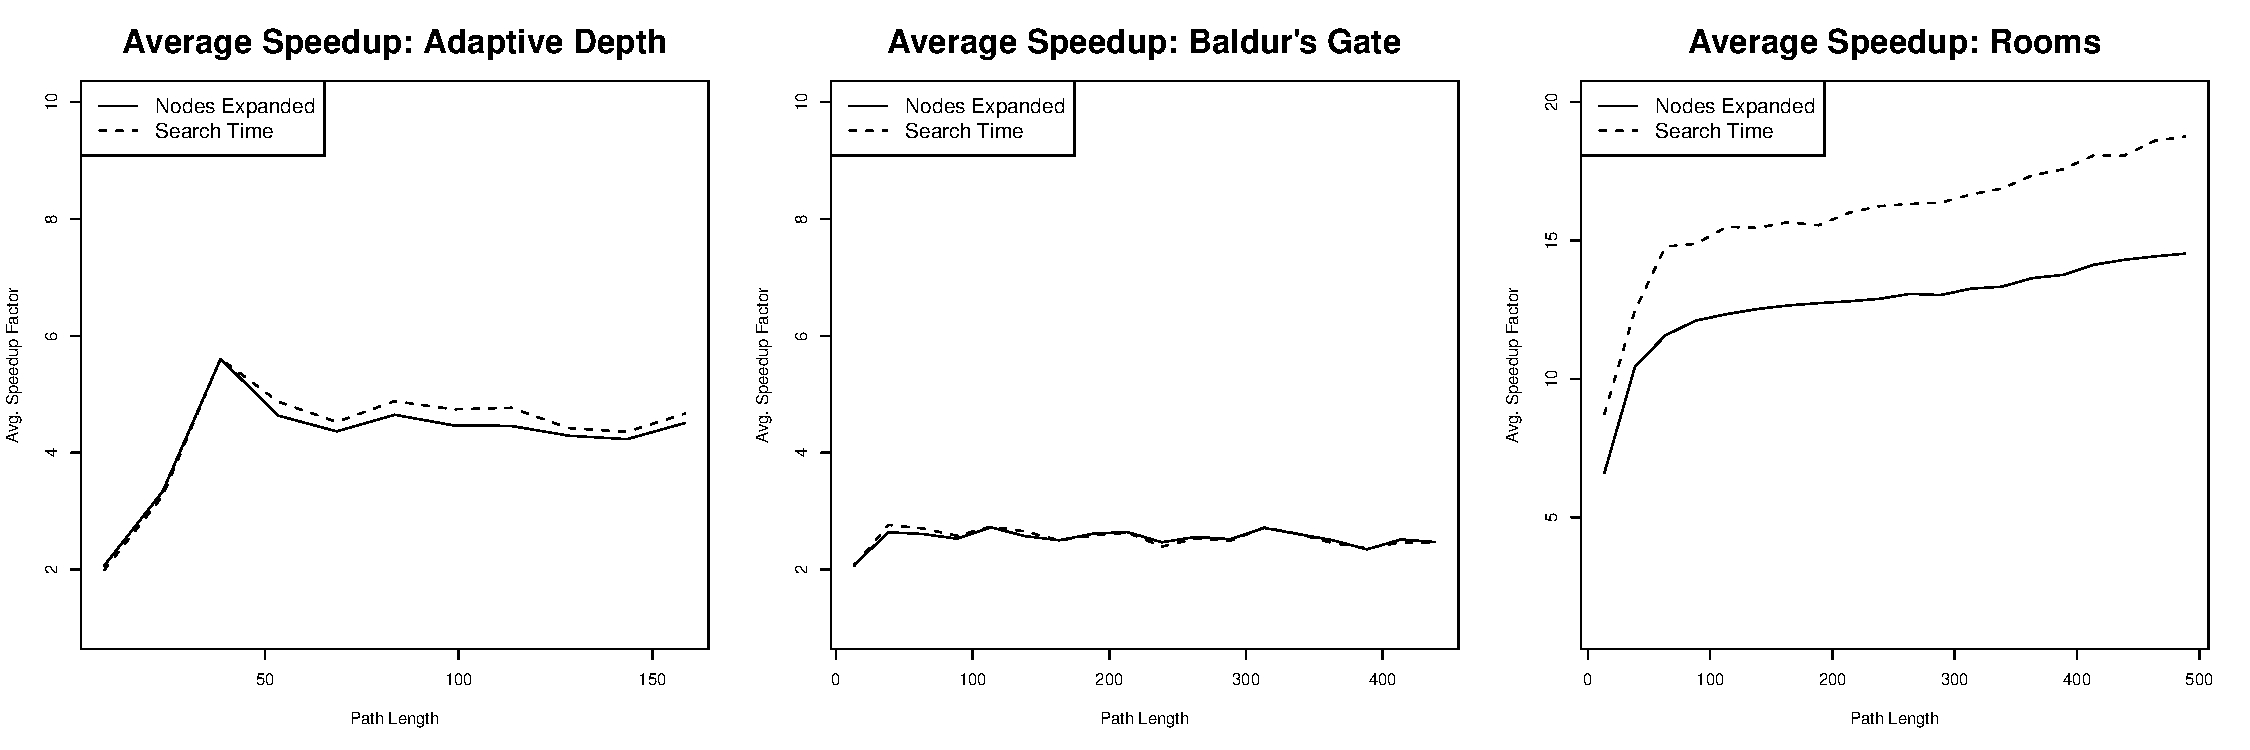
\includegraphics[width=0.8\textwidth, trim=20mm 0mm 40mm 0mm]{diagrams/speedup}
%\vspace{-1em}
%\caption{We manage to speed up A* by between 2-4 times on a range of synthetic
%and realistic benchmarks.}
%\end{center}
%\end{staticfigure}
%\end{staticcontents*}

\begin{staticcontents*}{nicta}
\begin{staticfigure}
\begin{center}

\includegraphics[width=2.5in]{diagrams/nicta_logo.jpg}
\end{center}
\end{staticfigure}
\end{staticcontents*}

\input problem
\input bigidea
\input results
\input futurework
\input moreinfo
%\bibliographystyle{plain}
%\bibliography{references}
\end{document}
